% ============================================================
%  future_as_anonymity.tex
%  Future Work: Extending the Proposed Scheme with
%               Authentication Server (AS) Anonymity
%
%  Author: Anup Kulkarni
%  IIT Guwahati — MTP Phase 2
%
%  Compile:  pdflatex future_as_anonymity
%            bibtex   future_as_anonymity
%            pdflatex future_as_anonymity
%            pdflatex future_as_anonymity
% ============================================================

\documentclass[12pt,a4paper]{article}

\usepackage[margin=2.5cm]{geometry}
\usepackage{amsmath,amssymb,amsthm}
\usepackage{booktabs}
\usepackage{multirow}
\usepackage{array}
\usepackage{tabularx}
\usepackage[table]{xcolor}
\usepackage{hyperref}
\usepackage{setspace}
\usepackage{parskip}
\usepackage{graphicx}
\graphicspath{{diagrams/}}
\usepackage{float}
\usepackage{caption}
\usepackage{subcaption}
\usepackage{enumitem}
\usepackage{mdframed}
\usepackage{tikz}
\usetikzlibrary{arrows.meta,positioning,calc,decorations.pathreplacing}

\onehalfspacing

\hypersetup{
  colorlinks=true,
  linkcolor=blue!60!black,
  citecolor=green!50!black,
  urlcolor=blue
}

% ---- Theorem-style environments ---------------------------
\newtheorem{theorem}{Theorem}[section]
\newtheorem{lemma}[theorem]{Lemma}
\newtheorem{property}{Property}[section]
\newtheorem{definition}{Definition}[section]

% ---- Custom commands for protocol notation ----------------
\newcommand{\IDd}{\mathit{ID}_D}
\newcommand{\IDas}{\mathit{ID}_{AS}}
\newcommand{\IDgw}{\mathit{ID}_{GW}}
\newcommand{\PID}{\mathit{PID}}
\newcommand{\PIDcurr}{\mathit{PID}_{\mathrm{curr}}}
\newcommand{\PIDown}{\mathit{PID}_{\mathrm{old}}}
\newcommand{\PIDnew}{\mathit{PID}_{\mathrm{new}}}
\newcommand{\PIDas}{\mathit{PID}_{AS}}
\newcommand{\PIDascurr}{\mathit{PID}_{AS}^{\mathrm{curr}}}
\newcommand{\PIDASOld}{\mathit{PID}_{AS}^{\mathrm{old}}}
\newcommand{\mcurr}{m_{\mathrm{curr}}}
\newcommand{\mold}{m_{\mathrm{old}}}
\newcommand{\mnew}{m_{\mathrm{new}}}
\newcommand{\KGWd}{K_{GW\text{-}D}}
\newcommand{\KGWas}{K_{GW\text{-}AS}}
\newcommand{\YASDhH}{Y_{AS\text{-}D}^{H}}
\newcommand{\YDH}{Y_D^{H}}
\newcommand{\SK}{\mathit{SK}}
\newcommand{\Rd}{R_D}
\newcommand{\cd}{c_D}
\newcommand{\yd}{y_D}
\newcommand{\TAcc}{T_{\mathit{Acc}}}
\newcommand{\authtoken}{\mathit{auth\_token}_D}
\newcommand{\etacurr}{\eta_{\mathrm{curr}}}
\newcommand{\etaold}{\eta_{\mathrm{old}}}
\newcommand{\rhoAS}{\rho_{AS}}
\newcommand{\Hf}{H(\cdot)}
\newcommand{\SE}{\mathit{SE}}
\newcommand{\PUF}{\mathit{PUF}}

\title{%
  \textbf{Extending Anonymity to Authentication Servers in
  Lightweight Decoupled IoT Authentication:}\\[4pt]
  \large A Scheme Design and Analysis\\[8pt]
  \normalsize\textit{MTP Future Work Document}%
}
\author{%
  Anup Kulkarni\\
  Roll No.\ 244101005\\[4pt]
  Under the Guidance of Dr.\ Manas Khatua\\[4pt]
  Department of Computer Science \& Engineering\\
  Indian Institute of Technology Guwahati\\
  Guwahati -- 781039, India
}
\date{June 2026}

\begin{document}
\maketitle
\tableofcontents
\newpage

% ============================================================
\section{Introduction and Motivation}
% ============================================================

\subsection{Background}

The proposed authentication scheme~\cite{das2026comsnets} introduces
\emph{device} anonymity into a lightweight, decoupled, distributed
authentication framework for multi-hop IoT networks.
Devices transmit a rotating pseudonym
$\PIDcurr = H(\IDd \,||\, \mcurr)$ in place of their real identity,
so no on-path observer --- including the gateway~(GW) --- learns~$\IDd$.
A dual-state mechanism~$(\PIDcurr, \PIDown, \mcurr, \mold)$ at the
Authentication~Server~(AS) handles lost key-exchange packets without
re-enrollment.

While device identity is fully shielded, the identity of the
\emph{Authentication Server} is not.
The current scheme transmits $\IDas$ in plaintext in the AS-to-GW
Phase~3 message, and embeds it inside a hash mask used during Phase~2.
A passive adversary monitoring the channel can therefore determine:
\begin{enumerate}
  \item which physical node is currently acting as AS, and
  \item which sessions that node authenticated (by correlating
        the AS-to-GW messages).
\end{enumerate}

This exposes the network topology.  In many IoT deployments ---
battlefield sensor nets, critical infrastructure monitoring,
healthcare body-area networks --- the identity of authentication
infrastructure nodes is itself sensitive.  If an adversary can
identify the AS, it becomes a high-value target for denial-of-service
or physical capture.

\subsection{Contribution of This Document}

This document proposes \textbf{AS~Pseudonym Rotation}: a minimal,
backward-compatible extension of the proposed scheme that assigns
each AS a rotating, epoch-bound pseudonym $\PIDas$ managed by the GW.
The key properties are:
\begin{enumerate}
  \item $\IDas$ never appears in plaintext on the open channel.
  \item Sessions authenticated by the same AS are unlinkable to a
        passive observer.
  \item The GW (and only the GW) can de-anonymize $\PIDas$ to
        recover~$\IDas$ --- accountability is preserved.
  \item A dual-state AS pseudonym mechanism handles epoch-transition
        desynchronization, mirroring the device desync mechanism.
  \item Communication overhead is limited to one additional 256-bit
        field ($\Psi$) in the Phase~3 AS-to-Device message.
\end{enumerate}

\subsection{Scope}

This document is a \emph{design and feasibility study}.
It is not a published paper; figures, protocol descriptions, and
security arguments are informal but rigorous.
Formal ProVerif verification is deferred as future work.

% ============================================================
\section{Related Work}
% ============================================================

\subsection{Infrastructure Pseudonymity in Vehicular Networks}

The most mature body of work on \emph{server-side} anonymity comes
from Vehicular-to-Infrastructure~(V2X) systems.
IEEE~1609.2~\cite{ieee16092} defines a pseudonym certificate framework
in which Road-Side Units~(RSUs) are assigned short-lived certificates
by a Pseudonym Certificate Authority (PCA).
Vehicles authenticate to an RSU using the RSU's current pseudonym
certificate; the certificate changes periodically so that long-term
vehicle--RSU associations cannot be built by observers.
Khodaei et al.~\cite{khodaei2018scaling} study the scalability of
this approach and show that GW-coordinated epoch changes with dual-state
overlap windows eliminate the need for vehicle-side re-registration
during certificate transitions.
The AS pseudonym scheme proposed here is structurally analogous:
the GW plays the role of the PCA, and the dual-state
$(\PIDascurr, \PIDASOld)$ mechanism mirrors the overlap window.

\subsection{Subscriber Identity Concealment in 5G}

The 3GPP 5G~SA specification (TS~33.501~\cite{3gpp33501}) introduces
the \emph{Subscriber Concealed Identifier}~(SUCI), which conceals the
long-term Subscriber Permanent Identifier~(SUPI) using the home network's
public key.
Although SUCI is asymmetrically encrypted rather than hash-based, the
functional goal is identical to our $\PIDas$: a one-use alias that
allows the network to authenticate the subscriber without transmitting
the permanent identity.
Importantly, only the Home Network (analogous to our GW) can recover
the SUPI from the SUCI.
Our construction is lighter: it uses only a shared secret and a
collision-resistant hash function, avoiding asymmetric operations that
are prohibitive on IoT hardware.

\subsection{Anonymity Taxonomy}

Pfitzmann and Hansen~\cite{pfitzmann2010terminology} define three
related notions relevant here.
\emph{Anonymity}: an agent cannot be identified within a set of
subjects.
\emph{Unlinkability}: two protocol runs cannot be associated with the
same subject.
\emph{Pseudonymity}: an agent uses a pseudonym instead of a true
identity, with possible de-pseudonymization by an authorised party.
The properties achieved by the proposed extension are:
\begin{itemize}
  \item \textbf{AS Anonymity} with respect to external observers
        (they see only~$\PIDas$).
  \item \textbf{Epoch-unlinkability} of AS across sessions: sessions
        in different epochs are unlinkable even if the observer can
        link sessions \emph{within} an epoch.
  \item \textbf{Accountable Pseudonymity}: the GW can always
        de-anonymize~$\PIDas$.
\end{itemize}

\subsection{Anonymity in IoT Authentication Schemes}

Most existing lightweight IoT authentication schemes protect
\emph{user/device} identity.
Ali and Ahmed~\cite{ali2024laaka} (LAAKA) use temporary identity tokens
that change per session.
Zhou et al.~\cite{zhou2024auth} mask the user ID inside an XOR expression.
He et al.~\cite{he2023lightweight} use a nonce-refreshed alias.
Alruwaili et al.~\cite{alruwaili2025raaf} (RAAF-MEC) conceal user
identity in a Mobile Edge Computing context.
\textbf{None of these schemes address the anonymity of the
authentication server or infrastructure node itself.}

The proposed scheme of Das and Khatua~\cite{das2026comsnets} is the
first in this class to address device anonymity through pseudonym
rotation; the present document extends it to cover AS anonymity,
achieving end-to-end anonymity for all entities except the GW itself.

% ============================================================
\section{Problem Statement: Where \texorpdfstring{$\IDas$}{ID\_AS} Leaks}
% ============================================================

\subsection{Original Scheme Message Flows}

Recall the four phases of the proposed scheme:
\begin{enumerate}
  \item \textbf{Enrollment} (D to AS via GW):
        GW assigns AS to device~D and communicates $\IDas$ to~D.
        AS stores $(y_D, \IDd, \PIDcurr, \PIDown, \mcurr, \mold,
        \KGWd, \KGWas, \TAcc)$.
        D stores $(y_D, \cd, \mcurr, \PIDcurr, \IDas)$.

  \item \textbf{Authentication} (D to AS):
        D computes
        $\YASDhH = H(y_D) \oplus H(\Rd \,||\, \mcurr \,||\, \PIDcurr
        \,||\, \IDas \,||\, ts_1)$
        and transmits $(\PIDcurr, \YASDhH, ts_1)$ to AS.

  \item \textbf{Key Exchange} (AS to D; AS to GW):
        \begin{itemize}
          \item AS$\to$D: $(m_H, ts_2)$ where
                $m_H = \mnew \oplus H(\YDH \,||\, \mcurr \,||\, \Rd' \,||\,
                \IDas \,||\, \PIDcurr \,||\, ts_2)$
          \item \textbf{AS$\to$GW:}
                $(\PIDnew, \underline{\IDas}, \authtoken)$
                where $\authtoken = \SE(\KGWas, (\KGWd \,||\, \IDas \,||\,
                \PIDnew \,||\, ts_{\mathit{auth}}))$
        \end{itemize}

  \item \textbf{Data Communication} (D to GW): uses session key $\SK$.
\end{enumerate}

\subsection{Identified Leakage Points}

\begin{mdframed}[backgroundcolor=yellow!10,linecolor=red!60!black,linewidth=1.2pt]
\textbf{Leakage~L1 (Plaintext transmission):}
The AS-to-GW Phase~3 message contains~$\IDas$ in \emph{cleartext}.
Any node on the path between AS and GW sees the real identity of the AS.

\textbf{Leakage~L2 (Hash embedding):}
$\IDas$ appears inside the hash mask in both Phase~2 and Phase~3.
While the hash itself is one-way, the value is used as a \emph{static}
component across all sessions.
An adversary who knows~$\IDas$ (e.g., from L1 in an earlier session)
can verify this association in future sessions.

\textbf{Leakage~L3 (Enrollment distribution):}
$\IDas$ is transmitted from GW to D during enrollment.
If the enrollment channel is not perfectly confidential, $\IDas$ leaks
at registration time.
\end{mdframed}

Leakage~L1 is the most damaging: it places $\IDas$ in the open in
\emph{every authenticated session}, allowing passive traffic analysis
to construct a complete map of which nodes serve as AS over time.

% ============================================================
\section{Extended Scheme: AS Pseudonym Rotation}
% ============================================================

\subsection{Design Principles}

The extension is governed by four principles:
\begin{enumerate}
  \item \textbf{Minimal change.} Only the fields involving~$\IDas$
        are modified.  The PUF-based secret derivation, hash accumulator,
        and device-side pseudonym mechanism are unchanged.
  \item \textbf{GW-managed epochs.}  The GW is the single point that
        knows the true identity of every AS.  It generates, distributes,
        and tracks AS pseudonyms.
  \item \textbf{Dual-state recovery.}  An AS pseudonym epoch change
        between enrollment and first authentication would desync the
        device's stored~$\PIDas$; dual-state storage at AS allows
        recovery without re-enrollment.
  \item \textbf{No new cryptographic primitives.}  Only hash functions
        and XOR operations are used, consistent with the original scheme.
\end{enumerate}

\subsection{New Notation}

Table~\ref{tab:notation} summarises the symbols introduced by this
extension.

\begin{table}[H]
\caption{New symbols introduced by the AS pseudonym extension.}
\label{tab:notation}
\centering
\renewcommand{\arraystretch}{1.3}
\begin{tabularx}{\textwidth}{@{}lX@{}}
\toprule
\textbf{Symbol} & \textbf{Meaning} \\
\midrule
$\etacurr, \etaold$ &
  GW-generated nonces for the current and previous AS pseudonym epoch \\
$\PIDascurr = H(\IDas \,||\, \etacurr)$ &
  Current AS pseudonym (computed and known only to GW and AS) \\
$\PIDASOld = H(\IDas \,||\, \etaold)$ &
  Previous AS pseudonym (for dual-state desync recovery) \\
$\Psi$ &
  Masked AS pseudonym update field sent in Phase~3 AS$\to$D message;
  $\Psi = \PIDascurr \oplus H(\KGWd \,||\, ts_2)$ \\
$\text{epoch}_{AS}$ &
  AS pseudonym epoch identifier (counter or timestamp, maintained by GW) \\
$\rhoAS$ &
  Long-term shared secret between GW and AS (used in key derivation) \\
\bottomrule
\end{tabularx}
\end{table}

For quick reference, Figure~\ref{fig:notation} gives a plain-language
glossary of every symbol used in the protocol diagrams that follow;
the shaded rows are the new elements introduced for AS anonymity.

\begin{figure}[H]
\centering
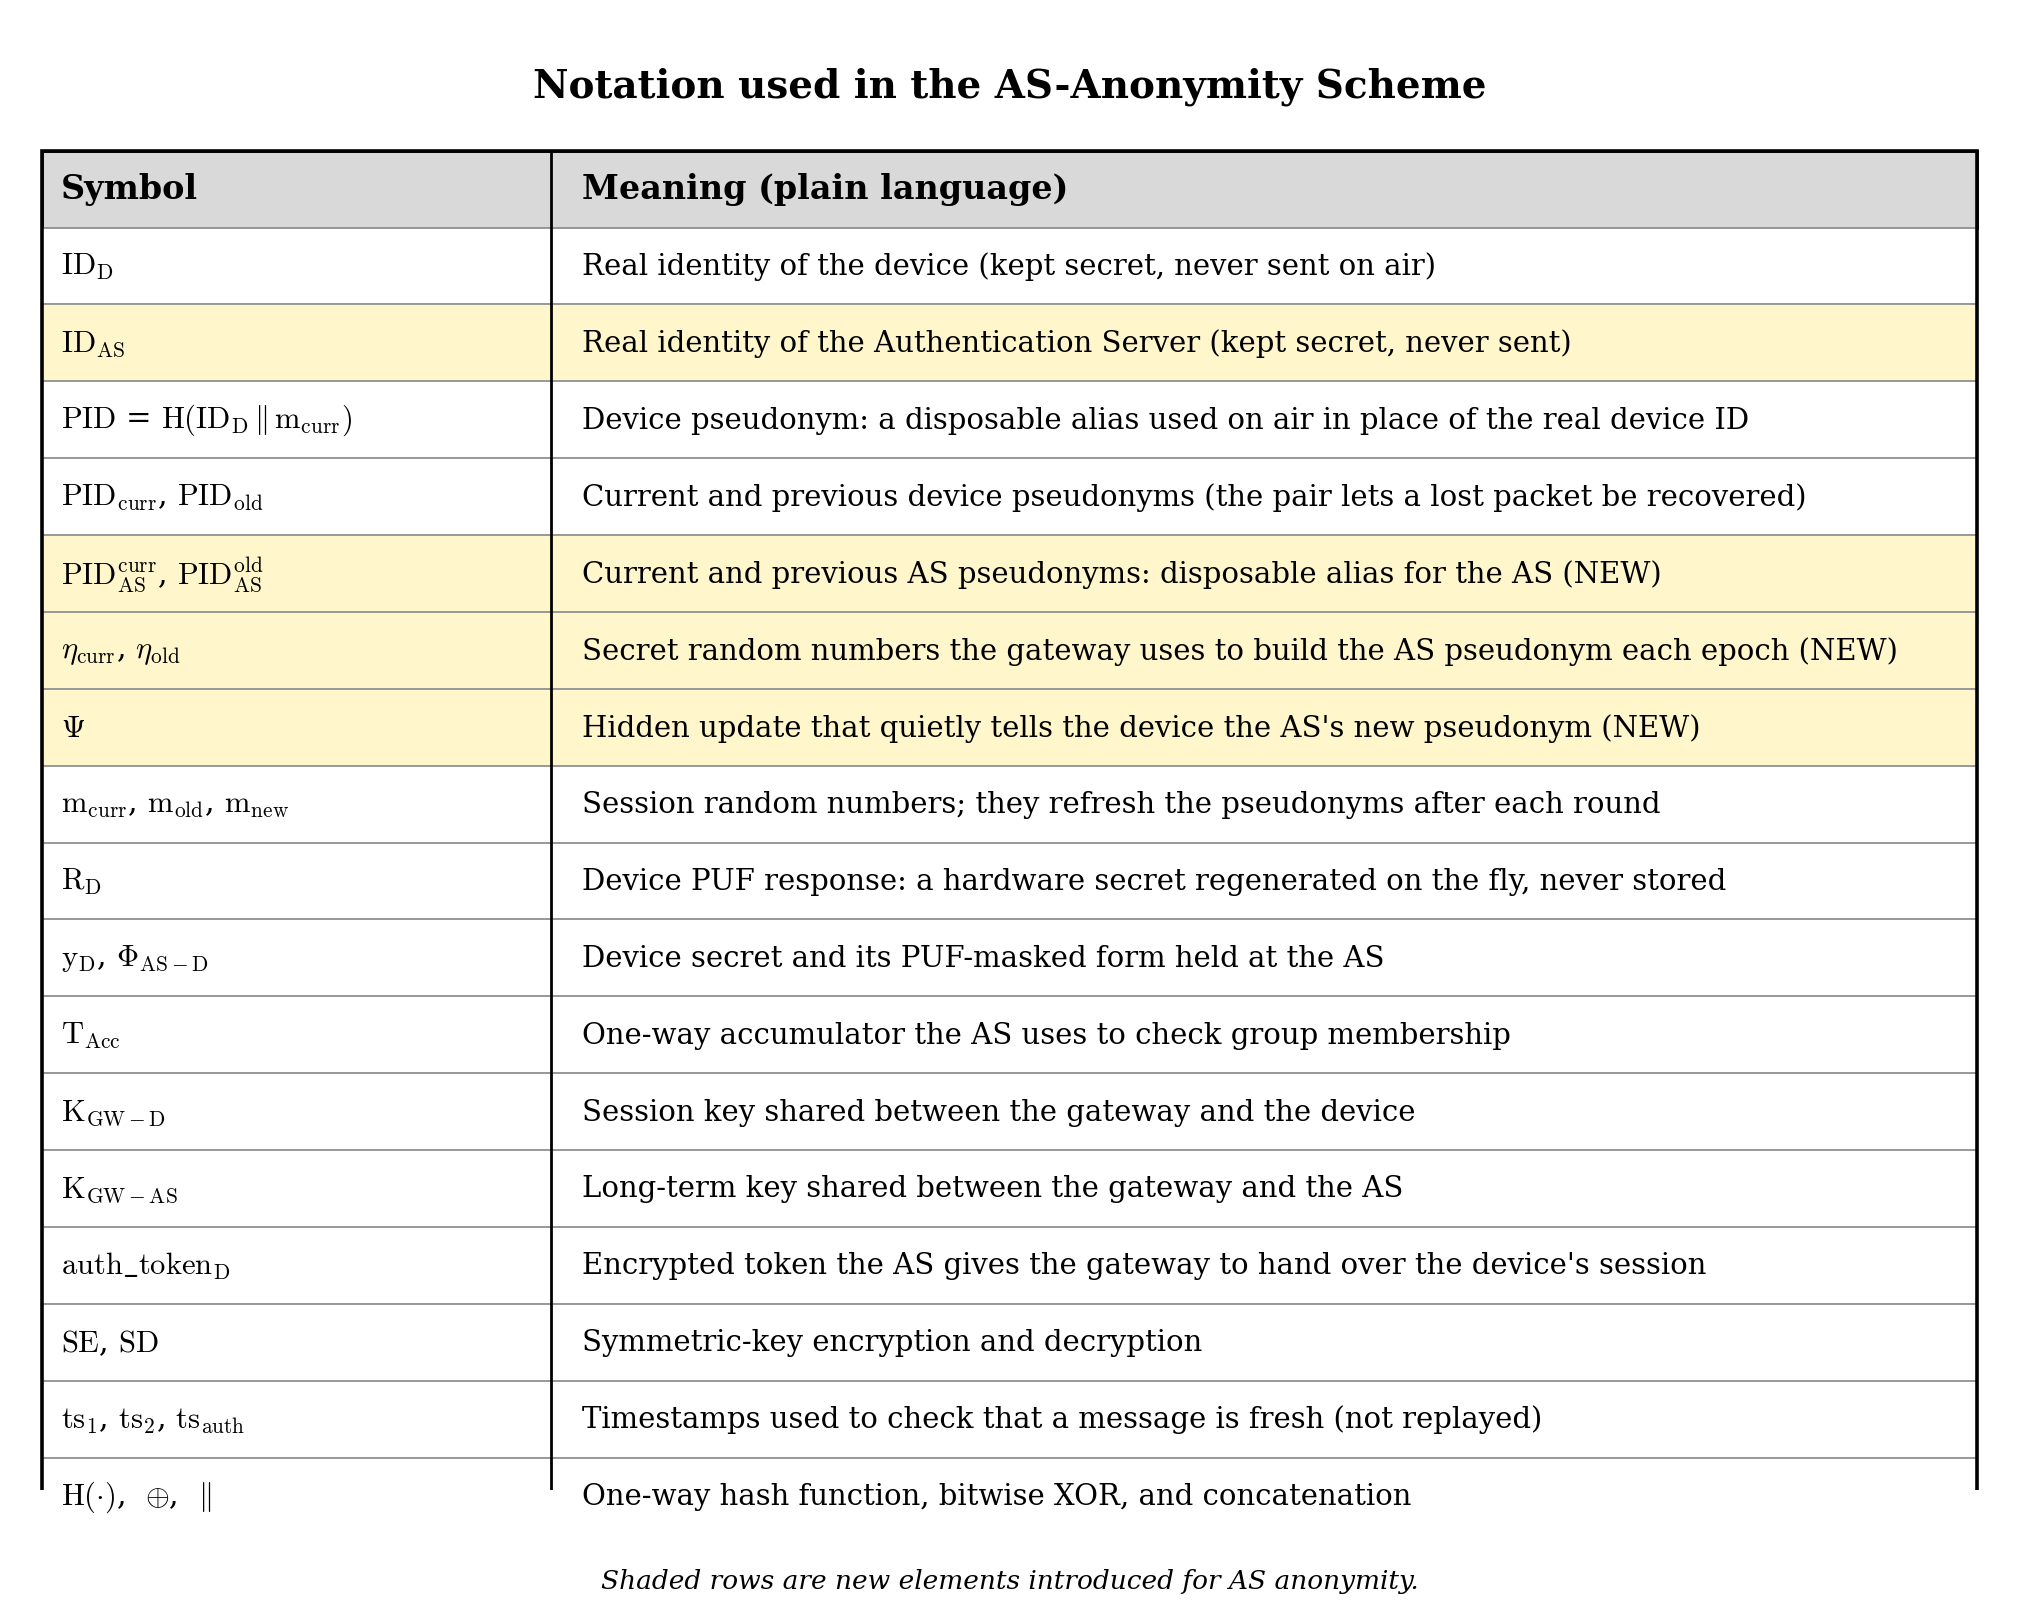
\includegraphics[width=\textwidth]{fig_future_notation.png}
\caption{Plain-language notation for the AS-anonymity scheme.
         Shaded rows mark the symbols added by this extension.}
\label{fig:notation}
\end{figure}

\subsection{Modified State Tables}

Tables~\ref{tab:state-gw}--\ref{tab:state-d} show the complete state
stored by each entity after the extension.

\begin{table}[H]
\caption{Extended GW state (additions highlighted).}
\label{tab:state-gw}
\centering
\renewcommand{\arraystretch}{1.3}
\begin{tabularx}{\textwidth}{@{}lX@{}}
\toprule
\textbf{Entity: GW} & \textbf{Stored per AS} \\
\midrule
$\IDas$           & Real identity of AS (GW-local, never transmitted) \\
$\KGWas$          & Long-term shared key with AS \\
\rowcolor{yellow!30}$\PIDascurr$   & Current AS pseudonym \\
\rowcolor{yellow!30}$\PIDASOld$    & Previous AS pseudonym \\
\rowcolor{yellow!30}$\etacurr, \etaold$ & Current and previous epoch nonces \\
\bottomrule
\end{tabularx}
\end{table}

\begin{table}[H]
\caption{Extended AS state (additions highlighted).}
\label{tab:state-as}
\centering
\renewcommand{\arraystretch}{1.3}
\begin{tabularx}{\textwidth}{@{}lX@{}}
\toprule
\textbf{Entity: AS} & \textbf{Stored} \\
\midrule
\multicolumn{2}{@{}l}{\textit{Per-device state (unchanged from original scheme):}} \\
$y_D, \IDd, \mcurr, \mold, \PIDcurr, \PIDown, \KGWd, \KGWas, \TAcc$ & (same as before) \\[4pt]
\multicolumn{2}{@{}l}{\textit{Own identity state:}} \\
$\IDas$                   & Real identity (local only) \\
\rowcolor{yellow!30}$\PIDascurr$  & Own current pseudonym (received from GW) \\
\rowcolor{yellow!30}$\PIDASOld$   & Own previous pseudonym (for reference in verification) \\
\bottomrule
\end{tabularx}
\end{table}

\begin{table}[H]
\caption{Extended Device state (additions highlighted).}
\label{tab:state-d}
\centering
\renewcommand{\arraystretch}{1.3}
\begin{tabularx}{\textwidth}{@{}lX@{}}
\toprule
\textbf{Entity: Device D} & \textbf{Stored} \\
\midrule
$y_D, \cd, \mcurr, \PIDcurr$ & (same as before) \\
\rowcolor{yellow!30}$\PIDascurr$ & Current pseudonym of assigned AS (replaces~$\IDas$) \\
\bottomrule
\end{tabularx}
\end{table}

\subsection{GW: AS Pseudonym Initialisation and Epoch Rotation}
\label{sec:epoch-rotation}

The GW manages AS pseudonym epochs independently of the session
protocol.  Epoch rotation is triggered by a time-based policy
(e.g., every 24~hours) or a count-based policy (every $N$~sessions).

\medskip
\noindent\textbf{Pseudonym Initialisation (at system bootstrap, per AS):}
\begin{enumerate}[label=\textbf{GW.\arabic*}]
  \item Generate fresh random nonce $\eta^{(0)}$.
  \item Compute $\PIDas^{(0)} = H(\IDas \,||\, \eta^{(0)})$.
  \item Transmit $\PIDas^{(0)}$ to AS over the existing secure channel
        (the same channel used for $\KGWas$ setup).
  \item Store $(\PIDascurr \leftarrow \PIDas^{(0)},\;
               \PIDASOld \leftarrow \bot,\;
               \etacurr  \leftarrow \eta^{(0)},\;
               \etaold   \leftarrow \bot)$.
  \item AS stores $(\PIDascurr \leftarrow \PIDas^{(0)},\;
                   \PIDASOld \leftarrow \bot)$.
\end{enumerate}

\noindent\textbf{Epoch Rotation (when epoch boundary is reached):}
\begin{enumerate}[label=\textbf{GW.\arabic*}]
  \item Generate fresh random nonce $\eta^{(k)}$.
  \item Compute $\PIDas^{(k)} = H(\IDas \,||\, \eta^{(k)})$.
  \item Transmit $\PIDas^{(k)}$ to AS over the secure channel.
  \item Update GW state:
        $\PIDASOld \leftarrow \PIDascurr,\;
         \PIDascurr \leftarrow \PIDas^{(k)},\;
         \etaold \leftarrow \etacurr,\;
         \etacurr \leftarrow \eta^{(k)}$.
  \item AS updates:
        $\PIDASOld \leftarrow \PIDascurr,\;
         \PIDascurr \leftarrow \PIDas^{(k)}$.
\end{enumerate}

\begin{mdframed}[backgroundcolor=blue!5]
\textbf{Invariant:}
At any moment, GW and AS agree on $(\PIDascurr, \PIDASOld)$.
A device enrolled during epoch $k-1$ stores $\PIDas^{(k-1)} =
\PIDASOld$ after epoch $k$ begins; the dual-state mechanism (Section~\ref{sec:desync})
handles this transparently.
\end{mdframed}

\subsection{Modified Phase 1: Enrollment}

The enrollment phase changes only in what the GW communicates to the
device about its assigned AS.

\medskip
\noindent\textbf{Modified step (GW to D):}

\emph{Old:} GW sends $\IDas$ and the AS's network address to~D.

\emph{New:} GW sends $\PIDascurr$ and the AS's network address to~D.

D stores $\PIDascurr$ in place of~$\IDas$.  D never learns the real
identity of its assigned AS.

All other enrollment steps (PUF challenge storage, hash accumulator
setup, $y_D$ derivation, AS state initialisation) are unchanged.
Figure~\ref{fig:enroll} shows the full modified enrollment message flow,
with the changed steps shaded.

\begin{figure}[H]
\centering
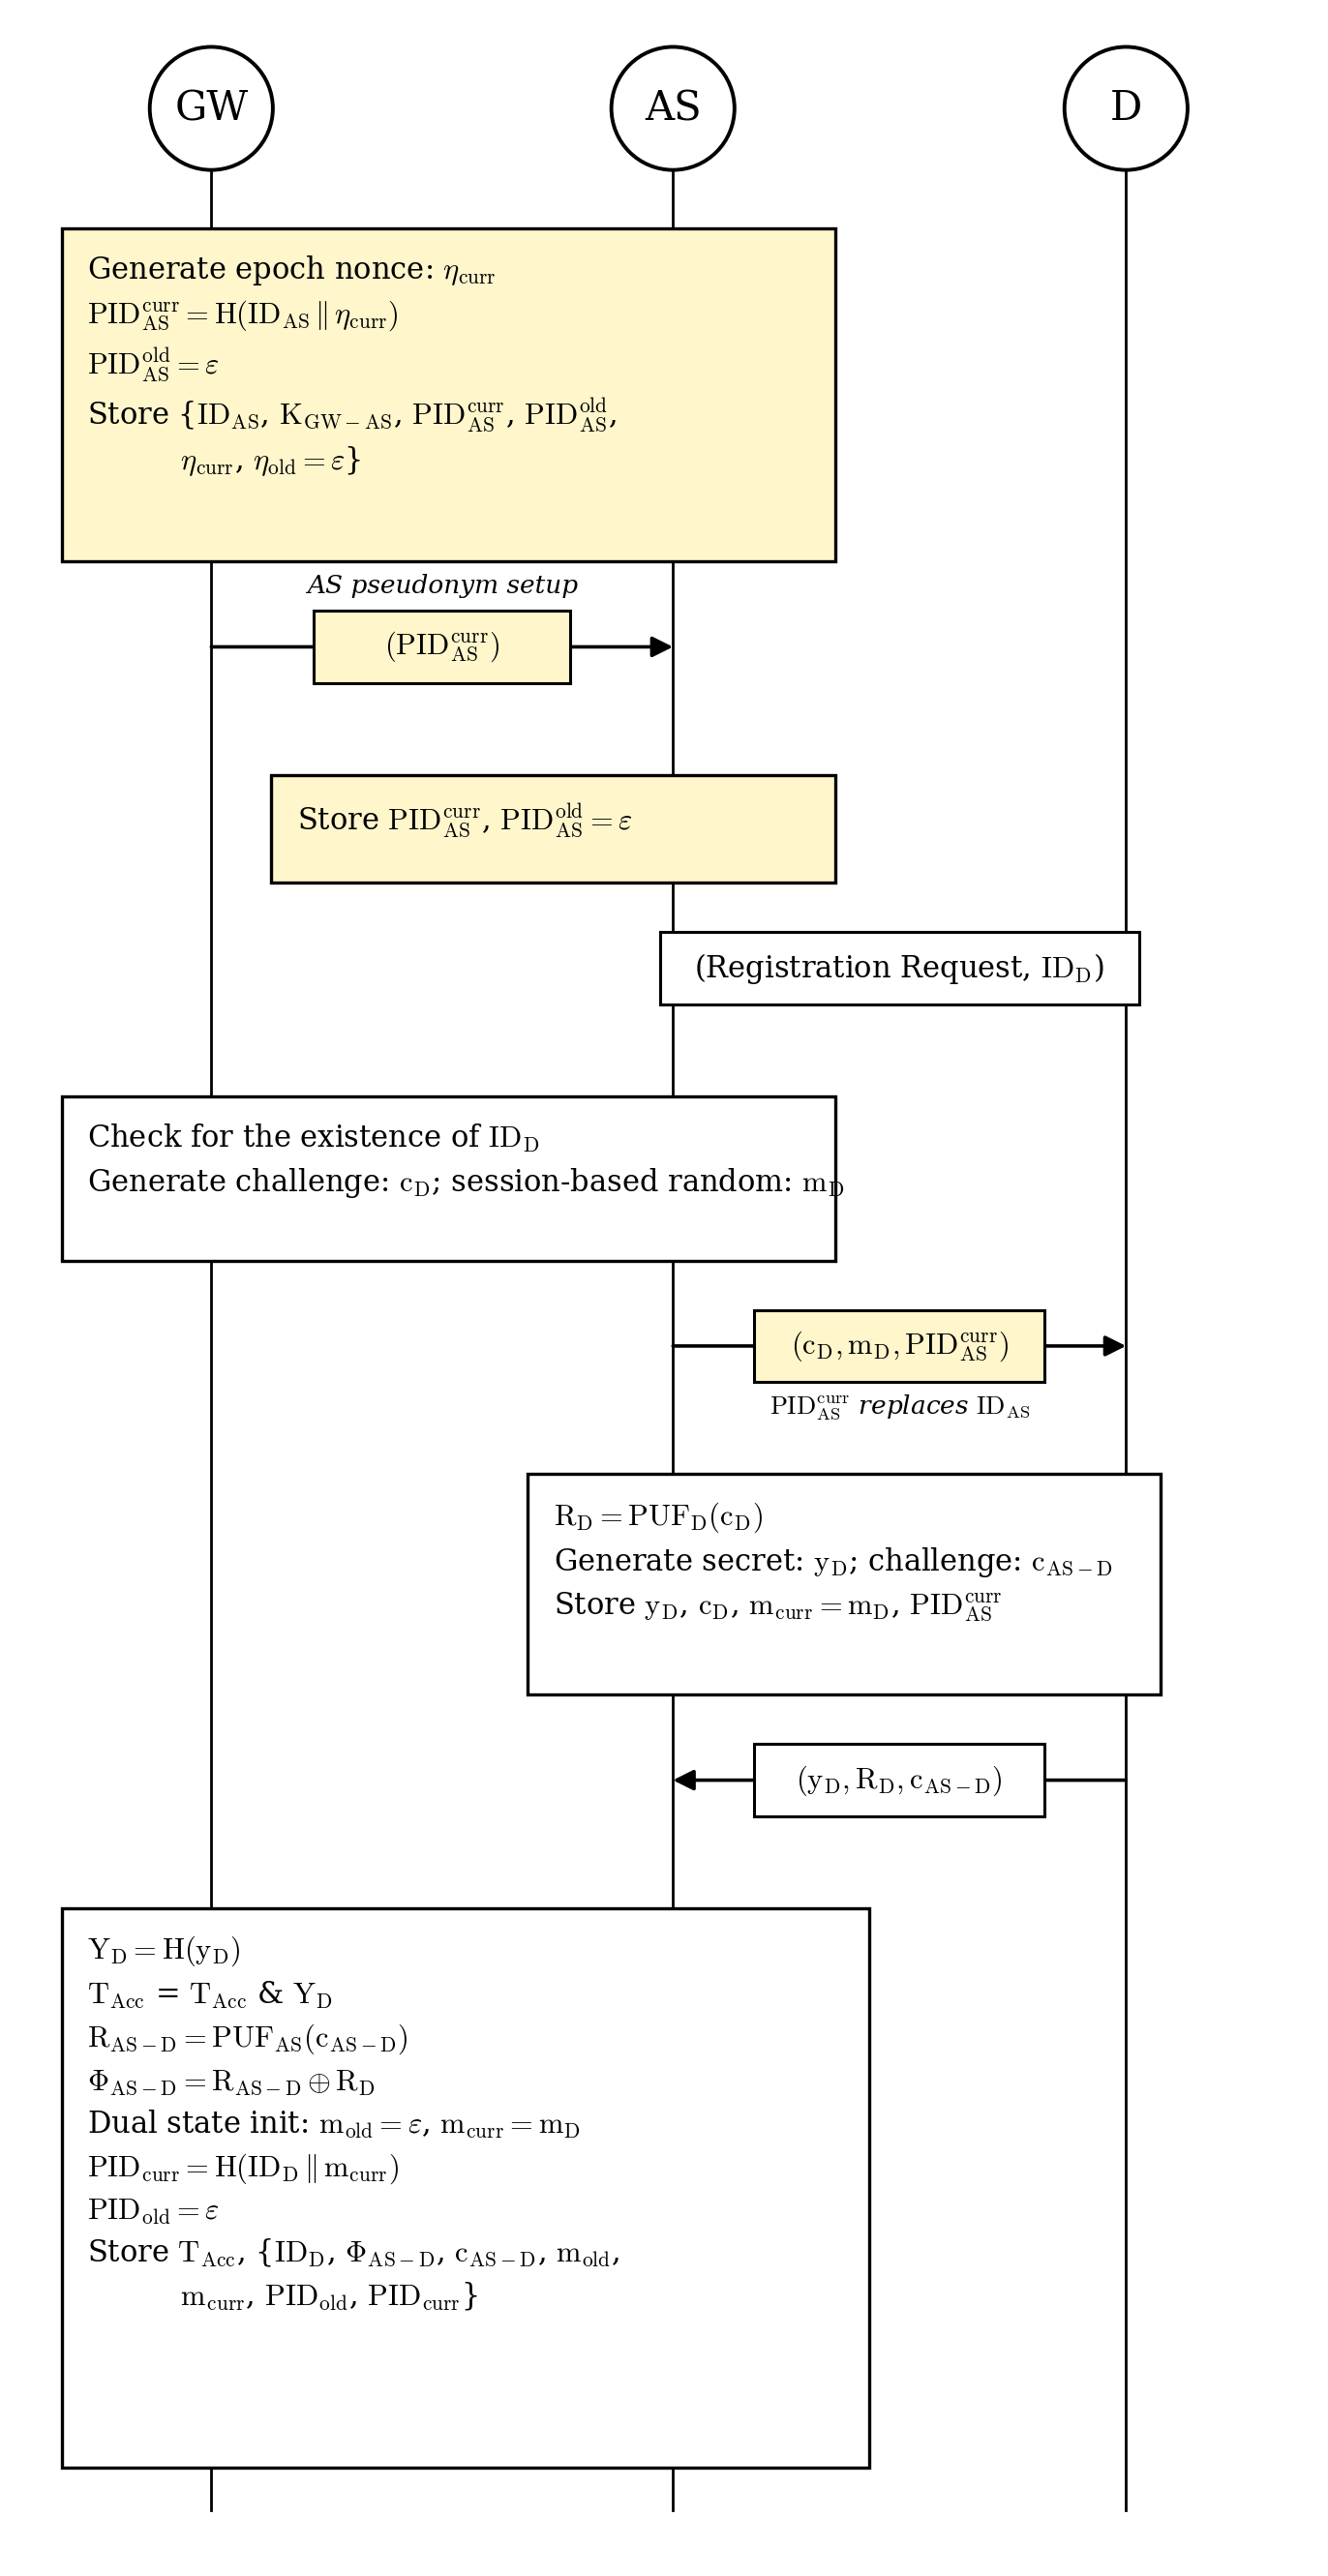
\includegraphics[width=0.92\textwidth]{fig_future_enrollment.png}
\caption{Modified enrollment phase.  The GW generates the epoch-bound
         AS pseudonym $\PIDascurr$ and delivers it to both AS and D;
         D stores $\PIDascurr$ in place of $\IDas$ (shaded steps are new).}
\label{fig:enroll}
\end{figure}

\subsection{Modified Phase 2: Authentication}
\label{sec:phase2-modified}

\noindent\textbf{D computes:}
\begin{equation}
  \YASDhH = H(y_D) \oplus H(\Rd \,||\, \mcurr \,||\, \PIDcurr \,||\,
  \underline{\PIDascurr} \,||\, ts_1)
  \tag{P2-D}
\end{equation}
(Previously: $H(\Rd \,||\, \mcurr \,||\, \PIDcurr \,||\,
\underline{\IDas} \,||\, ts_1)$.)

D transmits $(\PIDcurr, \YASDhH, ts_1)$ to AS. \textbf{Message format
unchanged.}

\medskip
\noindent\textbf{AS verifies:}
The original scheme tries two combinations of $(\mcurr, \mold)$ to
recover $H(y_D)$ and check membership in $\TAcc$.
The extended scheme must now also try two values of $\PIDas$, giving
four combinations.

AS iterates over:
\[
  \mathcal{V} = \{(\mcurr, \PIDascurr),\;
                   (\mcurr, \PIDASOld),\;
                   (\mold,  \PIDascurr),\;
                   (\mold,  \PIDASOld)\}
\]
in that order (most likely first).  For each $(m_{\mathrm{try}},
\PIDas^{\mathrm{try}})$:
\begin{align}
  Y_{\mathrm{try}} &= \YASDhH \oplus H(\Rd' \,||\, m_{\mathrm{try}} \,||\,
                     \PIDcurr \,||\, \PIDas^{\mathrm{try}} \,||\, ts_1)
                     \tag{P2-AS1}\\
  \text{Accept if} &\quad \TAcc \mathbin{\&} Y_{\mathrm{try}} = \TAcc
                     \tag{P2-AS2}
\end{align}
where $\Rd'$ is the PUF response AS holds for device~D (derived
during enrollment).  On acceptance, AS records the successful
$(m_D^{\mathrm{used}}, \PIDas^{\mathrm{used}})$ for use in Phase~3.

\begin{mdframed}[backgroundcolor=green!5]
\textbf{Complexity note:}
In the common case (no desync), only the first combination succeeds,
so there is no overhead.  In the worst case (both device nonce and AS
epoch are stale), all four are tried: three extra hash+XOR operations.
Given that IoT authentication is compute-limited by the network
round-trip, not local hashing, this is negligible.
\end{mdframed}

Figure~\ref{fig:auth} shows the full modified authentication phase,
including the four-way dual-state verification performed by the AS.

\begin{figure}[H]
\centering
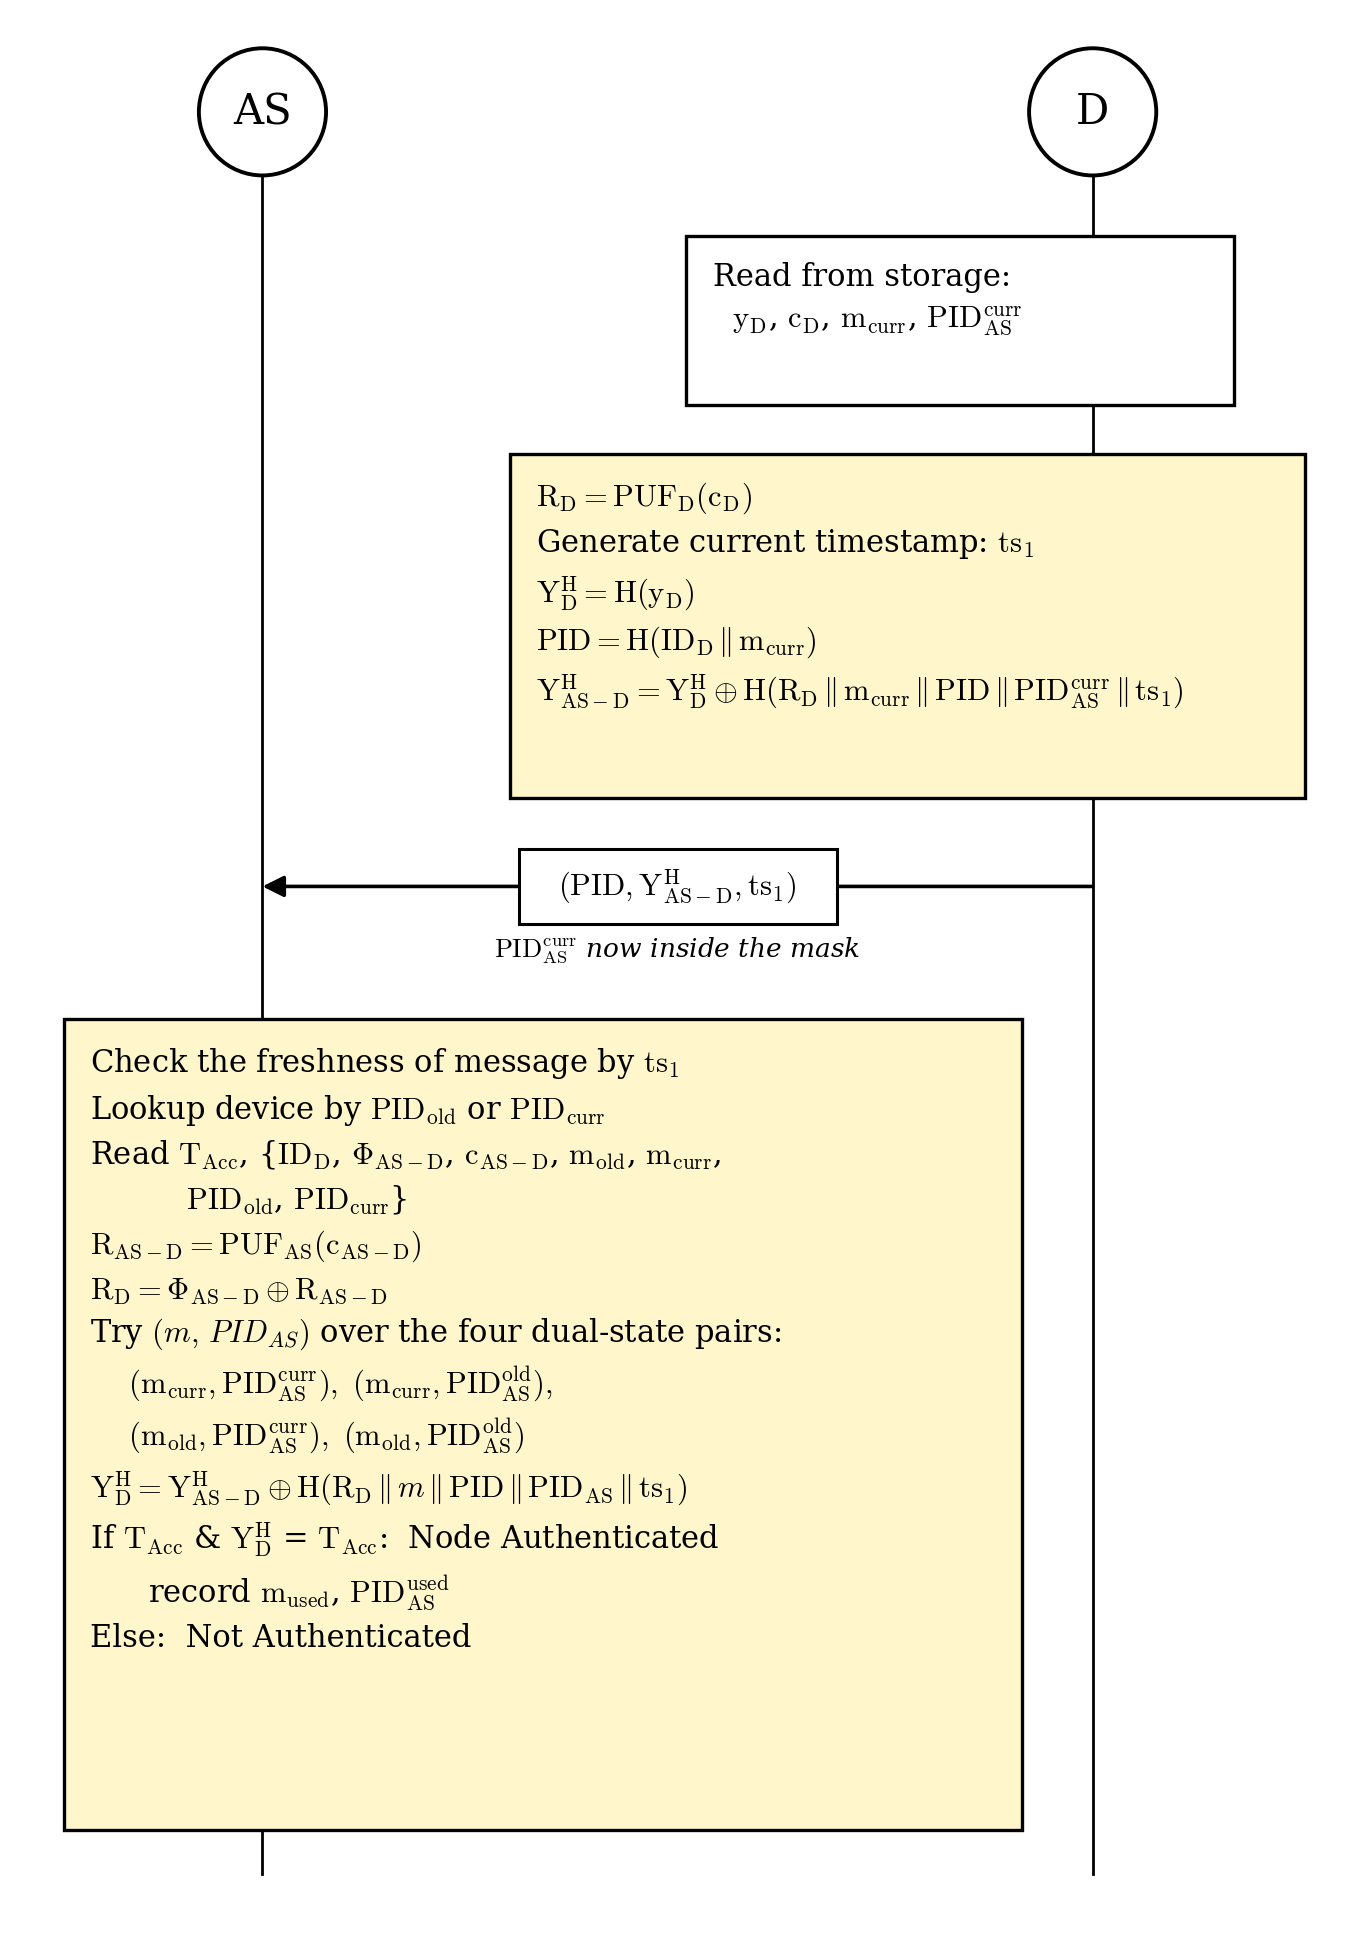
\includegraphics[width=0.92\textwidth]{fig_future_auth.png}
\caption{Modified authentication phase.  The device folds $\PIDascurr$
         into the verification mask, and the AS searches the four
         dual-state $(m, \PIDas)$ pairs until the accumulator check
         passes (shaded steps are new).}
\label{fig:auth}
\end{figure}

\subsection{Modified Phase 3: Key Exchange}
\label{sec:phase3-modified}

This is the primary modification.  Figure~\ref{fig:keyex-detail} gives
the detailed message flow with all computations, and the schematic in
Figure~\ref{fig:keyex-modified} highlights the boldface changes from the
original scheme.

\begin{figure}[H]
\centering
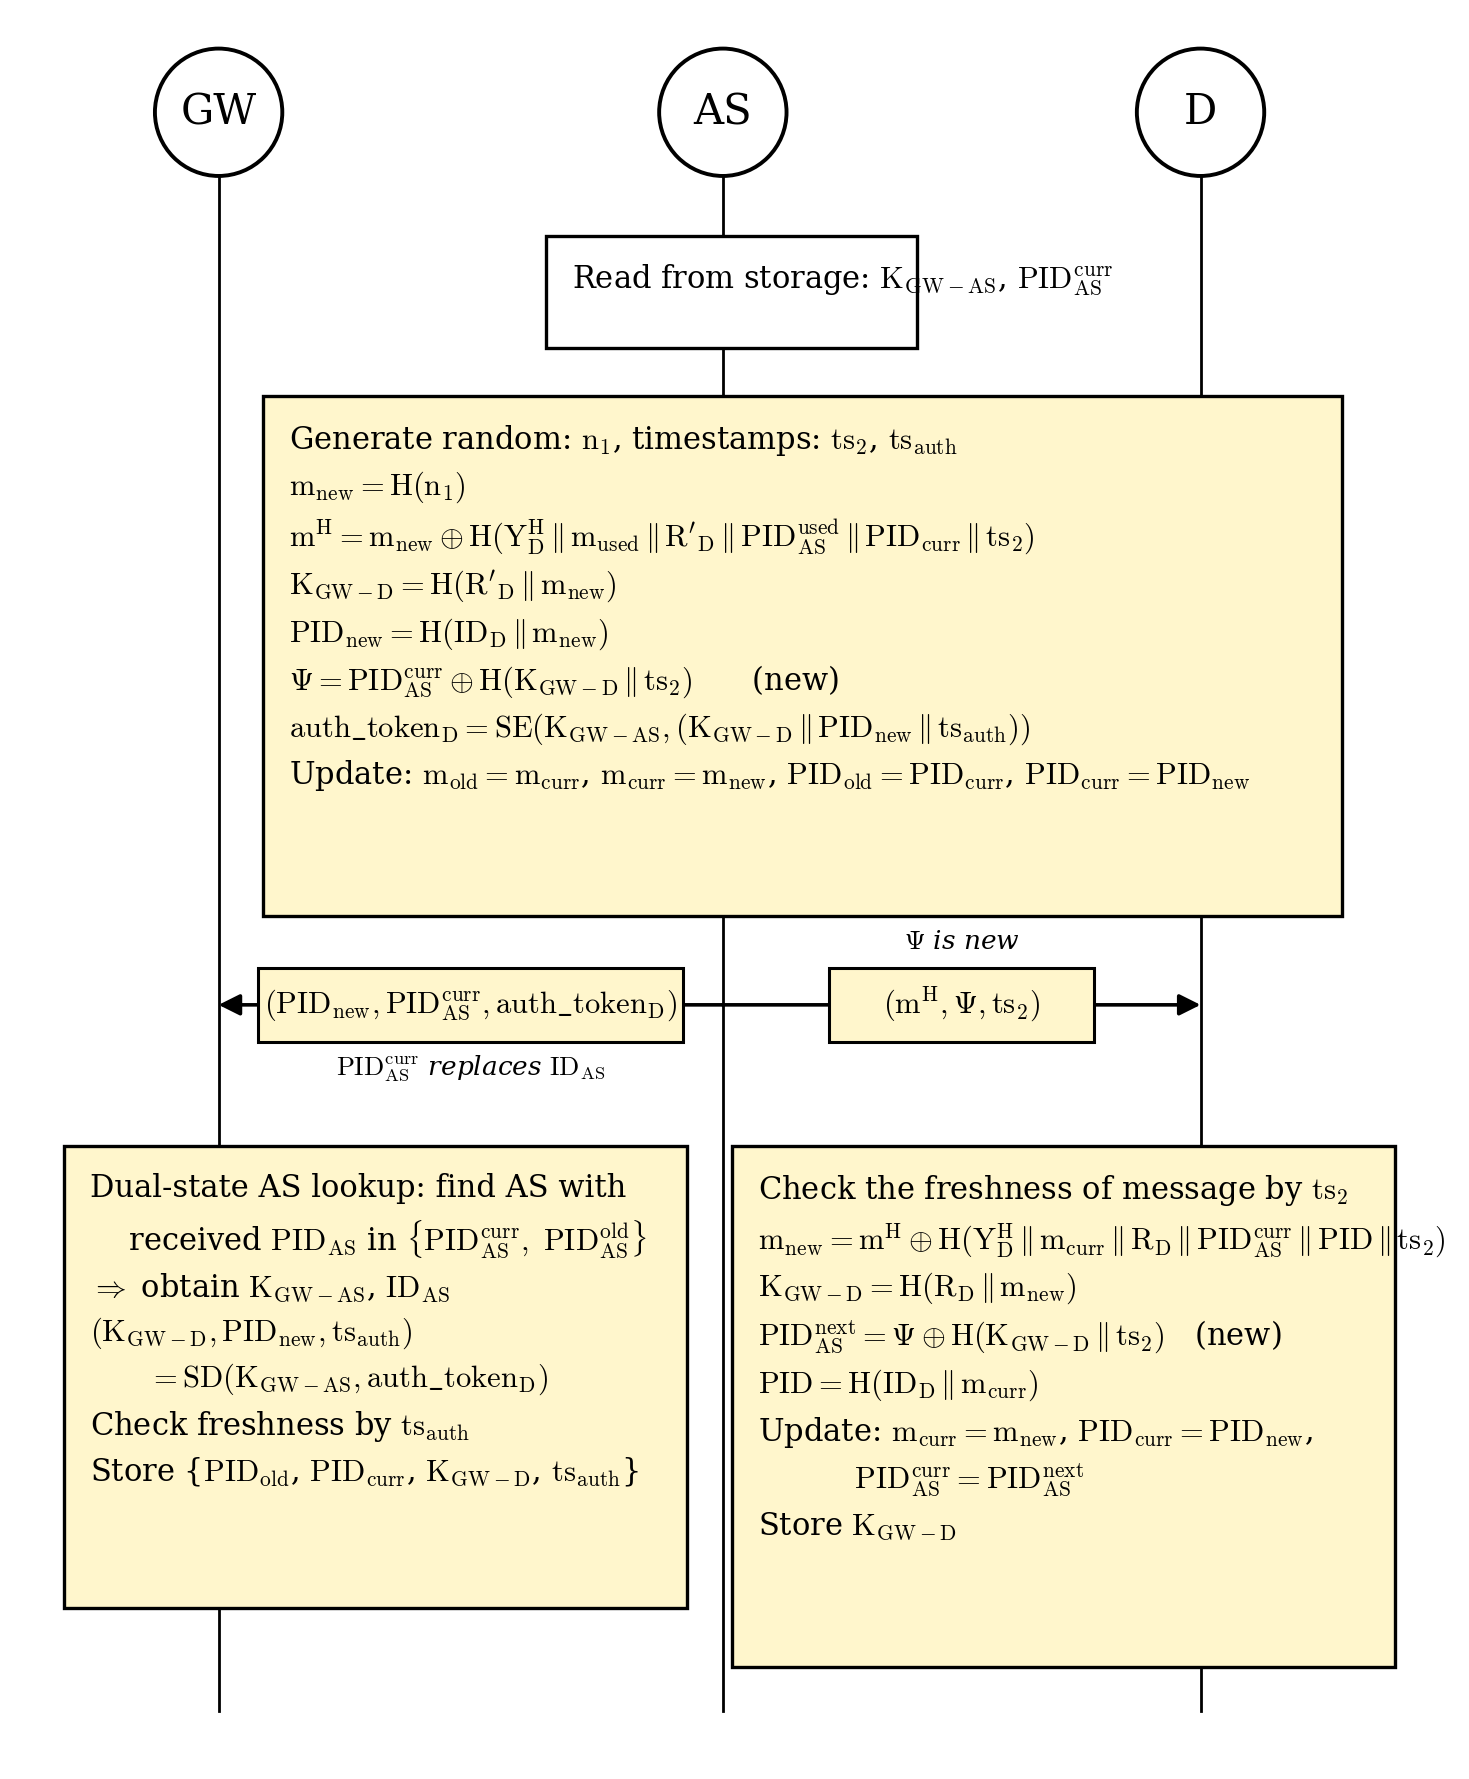
\includegraphics[width=\textwidth]{fig_future_keyex.png}
\caption{Modified key exchange phase (detailed).  AS adds the masked
         field $\Psi$ to refresh the device's stored AS pseudonym, and
         sends $\PIDascurr$ (not $\IDas$) to the GW; the GW resolves the
         AS via a dual-state pseudonym lookup (shaded steps are new).}
\label{fig:keyex-detail}
\end{figure}

\subsubsection*{AS Computes}
\begin{align}
  \mnew   &= H(n_1) \quad\text{(fresh nonce $n_1$ generated by AS)}
             \tag{P3-AS1}\\
  \KGWd   &= H(\Rd' \,||\, \mnew)
             \tag{P3-AS2}\\
  \PIDnew &= H(\IDd \,||\, \mnew)
             \tag{P3-AS3}\\
  m_H     &= \mnew \oplus H(\YDH \,||\, m_D^{\mathrm{used}} \,||\,
             \Rd' \,||\, \underline{\PIDas^{\mathrm{used}}} \,||\,
             \PIDcurr \,||\, ts_2)
             \tag{P3-AS4}\\
  \Psi    &= \PIDascurr \oplus H(\KGWd \,||\, ts_2)
             \tag{P3-AS5}\\
  \authtoken &= \SE(\KGWas,\; (\KGWd \,||\, \PIDnew \,||\,
               ts_{\mathit{auth}}))
               \tag{P3-AS6}
\end{align}
Note: $m_H$ uses $\PIDas^{\mathrm{used}}$ (the PID\_AS value D actually
had), while $\Psi$ always carries $\PIDascurr$ (the current epoch value,
which may or may not differ).

\medskip
\noindent\textbf{AS $\to$ D:} $\;(m_H,\; \Psi,\; ts_2)$
\hfill\textit{(added~$\Psi$)}

\medskip
\noindent\textbf{AS $\to$ GW:} $\;(\PIDnew,\; \underline{\PIDascurr},\;
\authtoken)$
\hfill\textit{($\IDas$ replaced by $\PIDascurr$)}

\subsubsection*{D Processes AS$\to$D}
\begin{align}
  \mnew   &= m_H \oplus H(\YDH \,||\, \mcurr \,||\, \Rd \,||\,
             \underline{\PIDascurr} \,||\, \PIDcurr \,||\, ts_2)
             \tag{P3-D1}\\
  \KGWd   &= H(\Rd \,||\, \mnew)
             \tag{P3-D2}\\
  \PIDas^{\mathrm{next}} &= \Psi \oplus H(\KGWd \,||\, ts_2)
             \tag{P3-D3}\\
  \PIDnew &= H(\IDd \,||\, \mnew)
             \tag{P3-D4}
\end{align}
D updates state: $\mcurr \leftarrow \mnew$,
$\PIDcurr \leftarrow \PIDnew$,
$\PIDascurr \leftarrow \PIDas^{\mathrm{next}}$.

\begin{mdframed}[backgroundcolor=blue!5]
\textbf{AS pseudonym consistency:}
If AS used $\PIDas^{\mathrm{used}} = \PIDASOld$ in $m_H$ (because D
had old~$\PIDas$), D uses its stored $\PIDascurr = \PIDASOld$ in
Eq.~(P3-D1) and correctly recovers~$\mnew$.
Then Eq.~(P3-D3) unmasks $\Psi = \PIDascurr^{\mathrm{new}} \oplus
H(\KGWd \,||\, ts_2)$ to give D the \emph{new} current pseudonym.
After step D3, D has the correct $\PIDascurr$ for the next session.
\end{mdframed}

\subsubsection*{GW Processes AS$\to$GW}
\begin{enumerate}[label=\textbf{GW.\arabic*}]
  \item Receive $(\PIDnew, \PIDas^{\mathrm{rcv}}, \authtoken)$.
  \item \textbf{Dual-state AS lookup:}
        Find AS such that $\PIDas^{\mathrm{rcv}} \in
        \{\PIDascurr, \PIDASOld\}$ for that AS.
        This yields~$\KGWas$ and~$\IDas$.
  \item Decrypt: $(\KGWd, \PIDnew', ts_{\mathit{auth}}) \leftarrow
        \SE^{-1}(\KGWas, \authtoken)$.
  \item Verify $\PIDnew = \PIDnew'$ and timestamp freshness.
  \item Store device session: $(D \mapsto (\PIDnew, \KGWd))$.
\end{enumerate}

\begin{figure}[H]
\centering
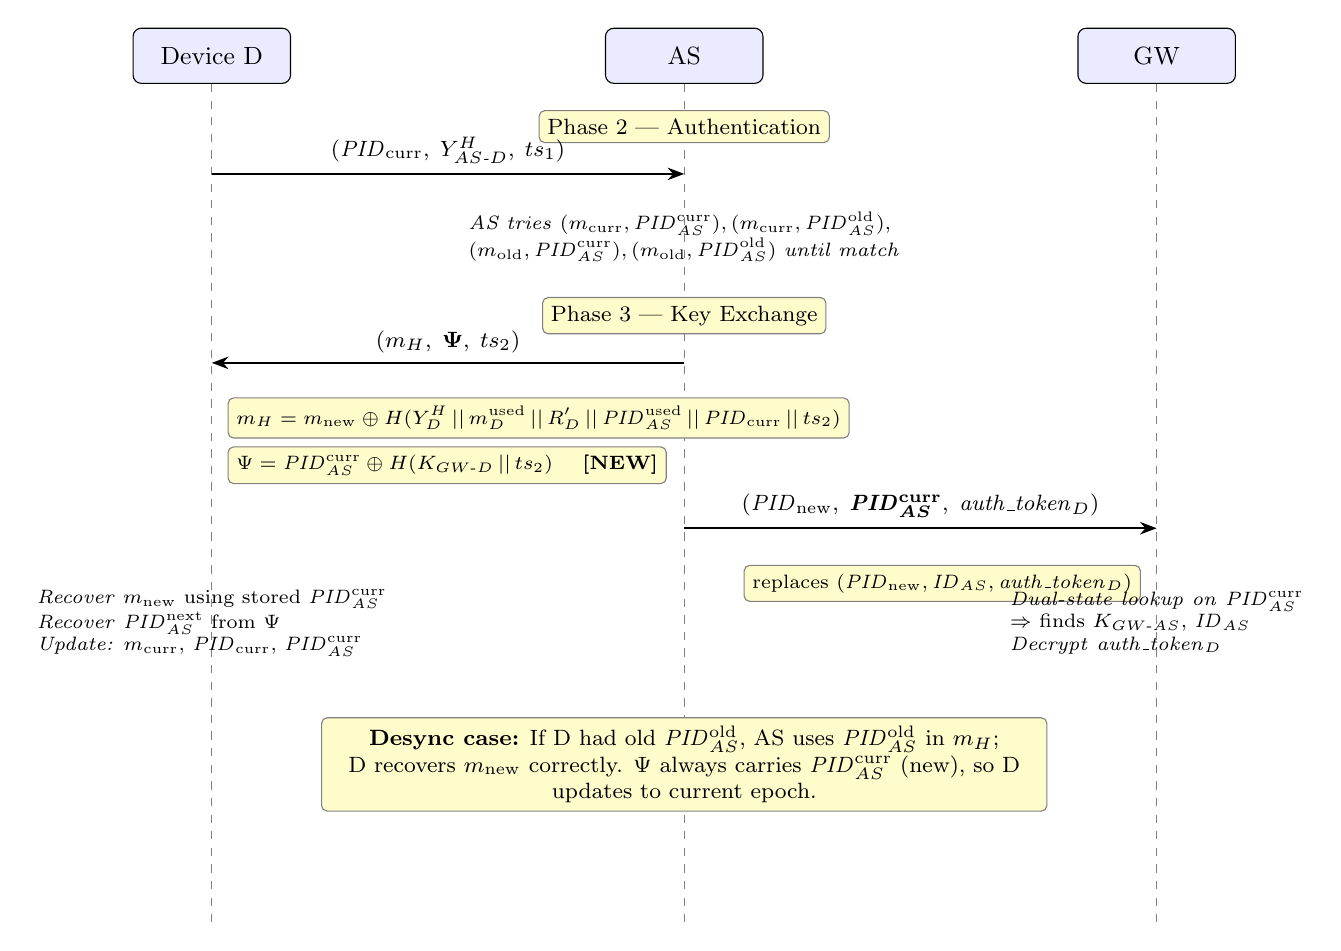
\begin{tikzpicture}[
  font=\small,
  box/.style={draw,rounded corners=3pt,fill=blue!8,
              minimum width=2.0cm,minimum height=0.7cm,
              text centered},
  arr/.style={-{Stealth[length=6pt]},thick},
  dasharr/.style={-{Stealth[length=6pt]},thick,dashed},
  lbl/.style={font=\footnotesize\itshape,midway},
  note/.style={font=\footnotesize,fill=yellow!20,draw=gray,
               rounded corners=2pt,inner sep=3pt}
]

% Entity boxes
\node[box] (D)  at (0,0)    {Device~D};
\node[box] (AS) at (6,0)    {AS};
\node[box] (GW) at (12,0)   {GW};

% Lifelines
\draw[gray,dashed] (D)  -- ++(0,-11);
\draw[gray,dashed] (AS) -- ++(0,-11);
\draw[gray,dashed] (GW) -- ++(0,-11);

% ---- Phase 2 ----
\node[note] at (6,-0.9) {Phase 2 — Authentication};

\draw[arr] (0,-1.5) -- (6,-1.5)
  node[lbl,above] {$(\PIDcurr,\; Y_{AS\text{-}D}^H,\; ts_1)$};

\node[align=left,font=\scriptsize] at (6,-2.3)
  {\textit{AS tries} $(\mcurr,\PIDascurr),(\mcurr,\PIDASOld),$\\
   $(\mold,\PIDascurr),(\mold,\PIDASOld)$ \textit{until match}};

% ---- Phase 3 ----
\node[note] at (6,-3.3) {Phase 3 — Key Exchange};

\draw[arr] (6,-3.9) -- (0,-3.9)
  node[lbl,above] {$(m_H,\; \boldsymbol{\Psi},\; ts_2)$};
\node[note,anchor=west] at (0.2,-4.6)
  {\scriptsize $m_H = \mnew \oplus H(Y_D^H \,||\, m_D^{\mathrm{used}} \,||\,
   R_D' \,||\, \PIDas^{\mathrm{used}} \,||\, \PIDcurr \,||\, ts_2)$};
\node[note,anchor=west] at (0.2,-5.2)
  {\scriptsize $\Psi = \PIDascurr \oplus H(\KGWd \,||\, ts_2)$
   \quad\textbf{[NEW]}};

\draw[arr] (6,-6.0) -- (12,-6.0)
  node[lbl,above] {$(\PIDnew,\; \boldsymbol{\PIDascurr},\; \authtoken)$};
\node[note,anchor=east] at (11.8,-6.7)
  {\scriptsize replaces $(\PIDnew, \IDas, \authtoken)$};

% D processes
\node[align=left,font=\scriptsize] at (0,-7.2)
  {\textit{Recover} $\mnew$ using stored $\PIDascurr$\\
   \textit{Recover} $\PIDas^{\mathrm{next}}$ from $\Psi$\\
   \textit{Update:} $\mcurr$, $\PIDcurr$, $\PIDascurr$};

% GW processes
\node[align=left,font=\scriptsize] at (12,-7.2)
  {\textit{Dual-state lookup on} $\PIDascurr$\\
   $\Rightarrow$ finds $\KGWas$, $\IDas$\\
   \textit{Decrypt} $\authtoken$};

% ---- Consistency note ----
\node[note] at (6,-9.0) {%
  \begin{minipage}{9cm}
  \centering
  \textbf{Desync case:} If D had old~$\PIDASOld$, AS uses $\PIDASOld$
  in~$m_H$;\\ D recovers $\mnew$ correctly.
  $\Psi$ always carries $\PIDascurr$ (new), so D updates to current epoch.
  \end{minipage}};

\end{tikzpicture}
\caption{Modified Phase~3 key exchange.  Boldface items are changed
from the original scheme.  GW lookup is now on~$\PIDascurr$ (not~$\IDas$);
D receives $\Psi$ to refresh its stored AS pseudonym.}
\label{fig:keyex-modified}
\end{figure}

\subsection{Dual-State AS Pseudonym Desynchronisation Recovery}
\label{sec:desync}

The dual-state mechanism for the AS pseudonym mirrors the existing
device-pseudonym mechanism.
Table~\ref{tab:desync-cases} enumerates all desync scenarios.

\begin{table}[H]
\caption{Desynchronisation scenarios and recovery paths.}
\label{tab:desync-cases}
\centering
\renewcommand{\arraystretch}{1.35}
\begin{tabularx}{\textwidth}{@{}p{4cm}p{4.5cm}X@{}}
\toprule
\textbf{Scenario} & \textbf{Root cause} & \textbf{Recovery} \\
\midrule
D has $m_{\mathrm{old}}$, current $\PIDascurr$
  & Phase~3 AS$\to$D lost; D did not update $\mcurr$
  & AS verifies with $(\mold, \PIDascurr)$; uses same in $m_H$;
    $\Psi$ confirms $\PIDascurr$ \\
\midrule
D has $\mcurr$, stale $\PIDASOld$
  & Epoch rotated after enrollment, before first auth
  & AS verifies with $(\mcurr, \PIDASOld)$; uses $\PIDASOld$ in $m_H$;
    $\Psi$ delivers $\PIDascurr$ (new) to~D \\
\midrule
D has $\mold$, stale $\PIDASOld$
  & Both: lost Phase~3 packet AND epoch rotation
  & AS verifies with $(\mold, \PIDASOld)$; $\Psi$ delivers $\PIDascurr$ \\
\midrule
D has $\mcurr$, current $\PIDascurr$
  & Normal (no desync)
  & AS verifies with $(\mcurr, \PIDascurr)$ (first try) \\
\bottomrule
\end{tabularx}
\end{table}

\noindent\textbf{Epoch window constraint:}
The GW must maintain $(\PIDascurr, \PIDASOld)$ for each AS, covering
exactly two consecutive epochs.  Devices that have been silent for
more than two epochs (i.e., missed two successive epoch rotations)
cannot recover via this mechanism and require re-enrollment.
This is acceptable since the epoch period should be set much longer
than the expected maximum idle period for any device.

% ============================================================
\section{Complete Modified Protocol Summary}
% ============================================================

For reference, Table~\ref{tab:protocol-diff} summarises every message
changed by the extension.

\begin{table}[H]
\caption{Per-message diff between original and extended scheme.}
\label{tab:protocol-diff}
\centering
\renewcommand{\arraystretch}{1.4}
\begin{tabularx}{\textwidth}{@{}lXX@{}}
\toprule
\textbf{Message} & \textbf{Original} & \textbf{Extended} \\
\midrule
GW$\to$D (enrollment)
  & $(\IDas, \mathit{addr}_{AS}, \ldots)$
  & $(\PIDascurr, \mathit{addr}_{AS}, \ldots)$ \\
\midrule
D$\to$AS (Phase~2 mask)
  & $H(\Rd \,||\, \mcurr \,||\, \PIDcurr \,||\, \IDas \,||\, ts_1)$
  & $H(\Rd \,||\, \mcurr \,||\, \PIDcurr \,||\, \PIDascurr \,||\, ts_1)$ \\
  & \multicolumn{2}{l}{\small\textit{(embedded in $\YASDhH$; wire format unchanged)}} \\
\midrule
AS$\to$D (Phase~3)
  & $(m_H, ts_2)$
  & $(m_H, \boldsymbol{\Psi}, ts_2)$ \quad +256~bit \\
\midrule
AS$\to$GW (Phase~3)
  & $(\PIDnew, \boldsymbol{\IDas}, \authtoken)$
  & $(\PIDnew, \boldsymbol{\PIDascurr}, \authtoken)$ \\
\midrule
Inside $\authtoken$
  & $\SE(\KGWas, (\KGWd \,||\, \IDas \,||\, \PIDnew \,||\, ts))$
  & $\SE(\KGWas, (\KGWd \,||\, \PIDnew \,||\, ts))$ \\
  & \multicolumn{2}{l}{\small\textit{(removing $\IDas$ from ciphertext;
    GW identifies AS via $\PIDascurr$ lookup)}} \\
\bottomrule
\end{tabularx}
\end{table}

% ============================================================
\section{Security Analysis}
% ============================================================

\subsection{AS Anonymity Against External Adversary}

\begin{property}[AS Anonymity]
\label{prop:as-anon}
A passive adversary observing all messages on all links cannot
determine the real identity~$\IDas$ of the authentication server
from the observed ciphertext.
\end{property}

\begin{proof}[Argument]
Every wire occurrence of the AS identity is either:
\begin{enumerate}
  \item Replaced by $\PIDascurr = H(\IDas \,||\, \etacurr)$ where
        $\etacurr$ is a GW-secret nonce.  Recovering $\IDas$ from
        $\PIDascurr$ requires inverting~$H$, which is computationally
        hard by the collision-resistance assumption.
  \item Inside the symmetric ciphertext $\authtoken$ encrypted under
        $\KGWas$ (now, only $\KGWd, \PIDnew, ts_{\mathit{auth}}$ are
        inside --- $\IDas$ has been removed from the ciphertext payload).
  \item Used only as a local variable inside AS and GW, never
        transmitted.
\end{enumerate}
Therefore no wire-level observation yields~$\IDas$.
\end{proof}

\subsection{Epoch-Unlinkability of AS Sessions}

\begin{property}[AS Epoch Unlinkability]
\label{prop:unlinkability}
Given two sessions $S_i$ and $S_j$ from different epochs $k$ and $k'$
($k \neq k'$), a computationally bounded adversary cannot determine
that they involved the same AS with probability better than
$\frac{1}{2} + \epsilon$ where $\epsilon$ is negligible.
\end{property}

\begin{proof}[Argument]
$\PIDas^{(k)} = H(\IDas \,||\, \eta^{(k)})$ and
$\PIDas^{(k')} = H(\IDas \,||\, \eta^{(k')})$.
Since $\eta^{(k)}$ and $\eta^{(k')}$ are independently drawn uniform
random nonces, the two pseudonyms are computationally independent.
An adversary distinguishing two sessions from the same AS must
link two independently uniform outputs of~$H$, which is infeasible
under the PRF assumption on~$H$.
\end{proof}

\textbf{Intra-epoch linkability:} Sessions within the same epoch use
the same $\PIDascurr$, so they \emph{are} linkable to the same AS
within that epoch.  This is an inherent trade-off: epochs must be
chosen short enough that linkability within an epoch is acceptable,
but long enough that epoch-rotation overhead is tolerable.
A 24-hour epoch with a busy AS authenticating 1000~devices per day
means at most 1000~sessions are linkable --- the same as in any
pseudonym-based system with a finite refresh period.

\subsection{AS Identity Secrecy (One-Way Pseudonym)}

\begin{property}[One-Way Pseudonym]
Given $\PIDascurr$, no PPT adversary can compute $\IDas$ without
knowing $\etacurr$.
\end{property}

This follows directly from the one-wayness of~$H$.
The adversary sees only $\PIDascurr$; $\etacurr$ is generated fresh
per epoch and stored only at the GW (never transmitted).

\subsection{Accountability: GW Can De-anonymise}

The GW stores $(\IDas, \PIDascurr, \PIDASOld, \etacurr, \etaold)$
for each AS.  Given any $\PIDas$ value from an observed message,
the GW can:
\begin{enumerate}
  \item Look up $\PIDas$ in its table to recover $\IDas$.
  \item Confirm: $\PIDas \stackrel{?}{=} H(\IDas \,||\, \etacurr)$
        or $H(\IDas \,||\, \etaold)$.
\end{enumerate}
This is exact, efficient, and requires no cryptographic inversion.
The GW can always hold the real AS accountable for any session.

\subsection{Forward Secrecy of AS Pseudonym}

If a past epoch nonce $\etaold$ is compromised (e.g., by storage
leakage at the GW), the adversary can recompute $\PIDASOld$ for the
affected AS.  However:
\begin{itemize}
  \item Future epochs use fresh, independently generated~$\eta$,
        so future $\PIDas$ values remain secure.
  \item Past sessions where $\PIDASOld$ was used are re-linkable, but
        no session key $\SK$ or device identity $\IDd$ is recovered
        (those are protected by separate mechanisms in the original
        scheme).
\end{itemize}
This is the standard forward-secrecy guarantee of epoch-based
pseudonym systems: compromise does not cascade to future epochs.

\subsection{Correctness Under Desynchronisation}

\begin{theorem}[Recovery Completeness]
\label{thm:desync}
Assuming the AS maintains dual-state $(\PIDascurr, \PIDASOld)$ and
epochs rotate at most once between two consecutive authentication
attempts by any device~D, the verification in
Section~\ref{sec:phase2-modified} always succeeds.
\end{theorem}

\begin{proof}
By case analysis on Table~\ref{tab:desync-cases}: all four combinations
of $(m_D^{\mathrm{used}} \in \{\mcurr, \mold\},\;
\PIDas^{\mathrm{used}} \in \{\PIDascurr, \PIDASOld\})$ are tried.
Since the epoch rotates at most once between D's last successful
authentication (when it updated its state) and the current attempt,
D's stored $\PIDas$ is at most one epoch stale, i.e., it equals
$\PIDASOld$.  Similarly, $m_D^{\mathrm{used}}$ is at most one
state behind.  Hence the correct combination is always in~$\mathcal{V}$,
and verification succeeds.
\end{proof}

\subsection{Preservation of Original Security Properties}

The extension does not alter:
\begin{itemize}
  \item The PUF-based secret derivation (device secret $\Rd$ is never
        stored or transmitted).
  \item The hash accumulator membership test ($\TAcc$).
  \item The device pseudonym rotation mechanism ($\PIDcurr, \PIDown$).
  \item The session key derivation ($\SK$, $\KGWd$).
  \item The ProVerif-verified properties Q1--Q14 of the original scheme:
        mutual authentication correspondences, session key secrecy,
        device anonymity ($\IDd$), and forward secrecy of~$m_{\mathrm{new}}$.
\end{itemize}
Property~Q15 (Device ID anonymity) continues to hold; the extension
adds a new property: AS ID anonymity.

% ============================================================
\section{Overhead Analysis}
% ============================================================

\subsection{Communication Overhead}

\begin{table}[H]
\caption{Communication overhead per authentication round
         (hash output = 256~bits; SE block = 256~bits).}
\label{tab:comm-overhead}
\centering
\renewcommand{\arraystretch}{1.3}
\begin{tabularx}{\textwidth}{@{}lrrX@{}}
\toprule
\textbf{Message} & \textbf{Original (bits)} & \textbf{Extended (bits)} & \textbf{Change} \\
\midrule
D$\to$AS (Phase~2)    & 768   & 768   & None (mask change internal) \\
AS$\to$D (Phase~3)    & 512   & 768   & $+256$ (new $\Psi$ field) \\
AS$\to$GW (Phase~3)   & 768   & 768   & None ($\PIDascurr$ same width as $\IDas$) \\
\midrule
\textbf{Total per round} & \textbf{2048} & \textbf{2304} & $+256$~bits (+12.5\%) \\
\bottomrule
\end{tabularx}
\end{table}

The overhead is modest: one additional 256-bit field~$\Psi$ in the
AS-to-Device message.  Out-of-band epoch rotation messages (GW~to~AS)
occur once per epoch and are negligible amortised over the epoch's
session count.

\subsection{Computation Overhead}

\begin{table}[H]
\caption{Hash (SHA-256 equivalent) and XOR operations added per round.}
\label{tab:comp-overhead}
\centering
\renewcommand{\arraystretch}{1.3}
\begin{tabularx}{\textwidth}{@{}lrX@{}}
\toprule
\textbf{Entity} & \textbf{Extra ops (worst case)} & \textbf{Description} \\
\midrule
Device D (Phase~2) & 0H + 0X & Mask uses $\PIDascurr$ instead of $\IDas$ \\
Device D (Phase~3) & +1H + 1X & Recover $\PIDas^{\mathrm{next}}$ from $\Psi$ \\
AS (Phase~2 verify) & +3H + 3X & Up to 3 extra verification attempts \\
AS (Phase~3 send)  & +1H + 1X & Compute $\Psi$ \\
GW (Phase~3)       & +0--1H  & Dual-state lookup (hash compare) \\
\midrule
\textbf{Total (worst)} & \textbf{+6H + 5X} & 6 extra SHA-256, 5 XOR \\
\midrule
\textbf{Total (normal)} & \textbf{+2H + 2X} & No desync \\
\bottomrule
\end{tabularx}
\end{table}

On Raspberry Pi 3B+, one SHA-256 operation on a 128-byte block
takes $\approx$0.02~ms.  Six extra hashes add at most $\approx$0.12~ms
to the AS's Phase~2 verification time --- well within the noise of
network latency on a multi-hop IoT network.

\subsection{Storage Overhead}

\begin{itemize}
  \item \textbf{GW (per AS):} $+2$ hash values ($\PIDascurr, \PIDASOld$)
        plus $+2$ nonces ($\etacurr, \etaold$) = $+128$~bytes.
  \item \textbf{AS (per device):} No change (device state unchanged).
        Own pseudonym state: $+2$ hash values = $+64$~bytes total at AS.
  \item \textbf{Device:} $\PIDascurr$ replaces $\IDas$; both are
        256-bit values.  Net change: zero.
\end{itemize}

The storage cost is concentrated at the GW, which is a capable node
and can afford it.  Device storage is unchanged.

% ============================================================
\section{Epoch Management Policy}
% ============================================================

The epoch rotation period $T_{\mathrm{epoch}}$ governs the
unlinkability--efficiency trade-off.

\paragraph{Short epochs ($T \approx 1$ hour).}
Strong unlinkability: each session window contains only
$\sim n_s$ sessions where $n_s$ is the session rate per hour.
Cost: frequent GW$\to$AS epoch rotation messages; higher likelihood
of desync for rarely-active devices.

\paragraph{Long epochs ($T \approx 1$ week).}
Minimal rotation overhead; low desync risk.
Cost: an adversary observing a week of traffic can correlate
all sessions to the same AS.

\paragraph{Recommended policy.}
Set $T_{\mathrm{epoch}}$ equal to the expected device sleep cycle
multiplied by a security margin of 2--4:
\[
  T_{\mathrm{epoch}} = 4 \times T_{\mathrm{sleep}}
\]
For typical IoT deployments with 15-minute sleep cycles,
$T_{\mathrm{epoch}} = 1$~hour.  This ensures that:
\begin{enumerate}
  \item A sleeping device waking up after one sleep cycle will not
        have missed more than one epoch rotation (given the margin).
  \item The adversary observing a single epoch window sees at most
        $\lfloor T_{\mathrm{epoch}} / T_{\mathrm{sleep}} \rfloor = 4$
        linkable sessions per AS.
\end{enumerate}

For deployments where devices can sleep for extended periods,
the GW should record the epoch at which each device last enrolled
or re-synchronized, and proactively send a re-enrollment invitation
if a device's stored epoch is more than two epochs stale.

% ============================================================
\section{Discussion}
% ============================================================

\subsection{Comparison with Device Pseudonym Mechanism}

Table~\ref{tab:comparison} contrasts the device and AS pseudonym
mechanisms.

\begin{table}[H]
\caption{Comparison of device and AS pseudonym mechanisms.}
\label{tab:comparison}
\centering
\renewcommand{\arraystretch}{1.3}
\begin{tabularx}{\textwidth}{@{}lXX@{}}
\toprule
\textbf{Property} & \textbf{Device pseudonym ($\PIDcurr$)} & \textbf{AS pseudonym ($\PIDascurr$)} \\
\midrule
Rotation trigger & Every successful session (Phase~3) & GW-initiated epoch rotation \\
Rotation authority & AS (computes $\PIDnew$) & GW (generates $\eta^{(k)}$) \\
De-anonymiser & AS knows $\IDd$ & GW knows $\IDas$ \\
Desync mechanism & $(m_{\mathrm{curr}}, m_{\mathrm{old}})$ dual-state at AS & $(\PIDascurr, \PIDASOld)$ dual-state at AS and GW \\
Update transmission & $m_H$ carries $\mnew$ encrypted & $\Psi$ carries $\PIDas^{\mathrm{next}}$ encrypted \\
Wire overhead added & None (replaces $\IDd$) & $+256$ bits ($\Psi$ field) \\
\bottomrule
\end{tabularx}
\end{table}

The key structural difference is that device pseudonyms rotate on
\emph{every session} (driven by the key-exchange protocol), while
AS pseudonyms rotate on \emph{epochs} (driven by the GW's policy).
This is appropriate because:
\begin{itemize}
  \item Device anonymity requires session-level unlinkability: an
        adversary observing consecutive packets should not link them
        to the same device.
  \item AS anonymity requires epoch-level unlinkability: an adversary
        observing traffic over a day/week should not identify which
        nodes are ASes.  Within an epoch, the AS identity is stable
        to allow efficient GW-side lookup.
\end{itemize}

\subsection{Complete Anonymity: Who Knows Whom}

After both extensions (device pseudonym from the original scheme +
AS pseudonym from this document), Table~\ref{tab:anon-summary}
summarises identity knowledge.

\begin{table}[H]
\caption{Identity knowledge matrix after full extension.}
\label{tab:anon-summary}
\centering
\renewcommand{\arraystretch}{1.35}
\begin{tabularx}{\textwidth}{@{}lXXX@{}}
\toprule
\textbf{Observer} & \textbf{Knows $\IDd$?} & \textbf{Knows $\IDas$?} & \textbf{Knows $\IDgw$?} \\
\midrule
Passive eavesdropper & No ($\PIDcurr$ only) & No ($\PIDascurr$ only) & GW is the trust anchor; identity assumed known \\
AS & Yes (enrolled) & Yes (own identity) & No (knows $\KGWas$ only) \\
GW & No (sees only $\PIDcurr$) & Yes (lookup table) & N/A \\
\bottomrule
\end{tabularx}
\end{table}

The GW remains the single privileged de-anonymiser for both devices
(via the $T_{\mathrm{Acc}}$ accumulator and Phase~3 decryption) and
ASes (via the pseudonym lookup table).  All other entities and all
passive observers have only pseudonymous handles.

\subsection{Open Questions for Future Formalisation}

\begin{enumerate}
  \item \textbf{ProVerif queries for AS anonymity:}
        A formal query
        $\mathtt{query\ attacker(ID_{AS})}$
        should be added to verify that the Dolev--Yao adversary cannot
        derive $\IDas$ from observed messages.
  \item \textbf{Intra-epoch unlinkability:}
        Within an epoch, sessions carry the same $\PIDascurr$.
        Formal unlinkability under a chosen-session attack model
        should be verified.
  \item \textbf{Epoch rotation authentication:}
        The GW-to-AS epoch rotation message (delivering $\PIDas^{(k)}$)
        uses the existing secure channel.  This channel's authentication
        mechanism should be formally modelled to ensure an adversary
        cannot inject a false epoch rotation.
  \item \textbf{Multi-AS scenario:}
        If a device migrates to a new AS (e.g., due to GW re-assignment),
        a new enrollment sub-protocol is needed.  The interaction between
        device pseudonym state and AS pseudonym state during migration
        is a non-trivial design problem.
\end{enumerate}

% ============================================================
\section{Conclusion}
% ============================================================

This document has presented a concrete scheme extension that closes
the AS identity leakage present in the proposed lightweight IoT
authentication scheme.
The core idea --- replacing $\IDas$ with an epoch-bound GW-managed
pseudonym $\PIDas$ --- is simple, requires no new cryptographic
primitives, and adds only one hash-and-XOR operation on the device
side and one 256-bit field ($\Psi$) to the AS-to-Device message.

The extension achieves AS anonymity and epoch-level unlinkability
against passive adversaries while preserving full accountability
at the GW.  A dual-state $(\PIDascurr, \PIDASOld)$ mechanism handles
epoch-transition desynchronisation in all four possible desync
scenarios without requiring re-enrollment.

The overhead is modest: $+256$~bits of communication per authentication
round, $\sim+6$ hash operations in the worst case, and $+128$~bytes
of GW storage per AS.  These costs are negligible relative to the
security gain.

The design is ready for ProVerif formalisation and prototype
implementation as a natural continuation of the current MTP work.

% ============================================================
%  Bibliography
% ============================================================
\bibliographystyle{IEEEtran}
\bibliography{ref}

\end{document}
